\documentclass[9pt]{IEEEtran}

\usepackage[english]{babel}
\usepackage{graphicx}
\usepackage{epstopdf}
\usepackage{fancyhdr}
\usepackage{amsmath}
\usepackage{amsthm}
\usepackage{amssymb}
\usepackage{url}
\usepackage{array}
\usepackage{textcomp}
\usepackage{listings}
\usepackage{hyperref}
\usepackage{xcolor}
\usepackage{colortbl}
\usepackage{float}
\usepackage{gensymb}
\usepackage{longtable}
\usepackage{supertabular}
\usepackage{multicol}
\usepackage{tabu}
\usepackage{verbatim}

\usepackage[utf8x]{inputenc}

\usepackage[T1]{fontenc}
\usepackage{lmodern}
\input{glyphtounicode}
\pdfgentounicode=1

\usepackage{fancyvrb}
\DefineVerbatimEnvironment{Code}{BVerbatim}{baseline=t}


\DeclareGraphicsExtensions{.pdf,.png,.jpg,.eps}

% correct bad hyphenation here
\hyphenation{op-tical net-works semi-conduc-tor trig-gs}

% ============================================================================================

\title{\vspace{0ex}
Data Extractor}

\author{Timotej Kovač\vspace{-4.0ex}}

% ============================================================================================

\begin{document}

\maketitle

\section{Introduction}

In this paper we provide and discuss results gathered when trying to implement data extraction algorithms using regular expressions, XPath and automatic web extraction.
The later was implemented using RoadRunner approach for automatic web extraction~\cite{roadrunner}, though the algorithm does not strictly follow their implementation approach but rather uses their general observations.


\section{Selection of optional web pages}

For our first website we have chosen a detailed description page of a product available on web store Mimovrste~\cite{mimovrste}.
Here we have chosen some interesting fields that we might be useful as shown in figure ~\ref{fig_mimovrste}.
These were:
\begin{itemize}
\item{\textbf{TAGS*}, which further describe the item as having a discount, being a recommended product, etc.";}
\item{\textbf{TITLE};}
\item{\textbf{DESCRIPTION};}
\item{\textbf{OLD PRICE*}, which states the price before the now discounted price;}
\item{\textbf{PRICE}, which states the current price;}
\item{\textbf{SAVINGS*}, which represents the percentage saved;}
\item{\textbf{AVAILABILITY}, which states when the product will be available for shipment.}
\end{itemize}
Fields above marked with an asterisk don't appear always and are therefore optional.

\begin{figure}[ht]
    \centering
    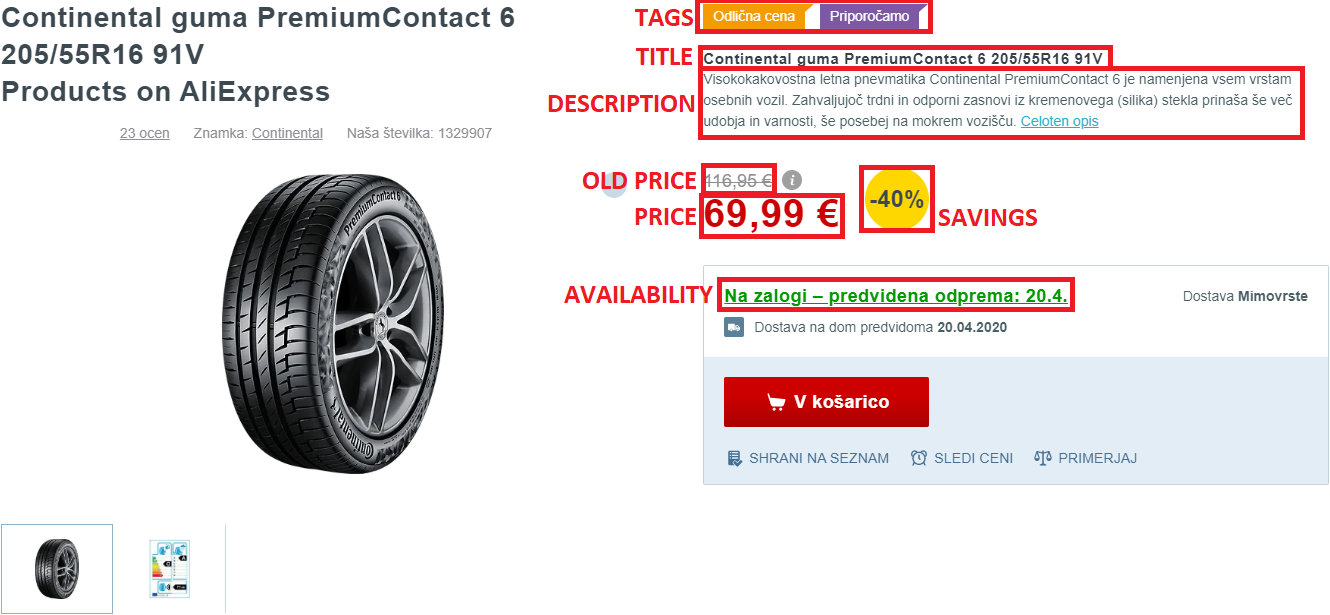
\includegraphics[width=1\columnwidth]{mimovrste.png}
    \caption{Web store mimovrste.si with tagged fields that we used for extraction of web content.}
    \label{fig_mimovrste}
\end{figure}

For our second website we have chosen a page containing multiple items in a grid pattern on a web site Ceneje~\cite{ceneje}.
Here we have chosen the fields listed bellow:
\begin{itemize}
\item{\textbf{IMAGE};}
\item{\textbf{TITLE};}
\item{\textbf{MIN PRICE}, which states the minimal price in all of the stores that provide the product;}
\item{\textbf{NUMBER OF STORES}, which states the number of stores that provide the product;}
\item{\textbf{ACTION}, which states what the button does either takes the user to a particular web store or to a list of web stores still on the same ceneje.si domain.}
\end{itemize}
Here none of the fields are optional but some do vary as they may contain some other words in front of the fields or are ads which have a slightly different structure.
This too can be seen in figure~\ref{fig_ceneje}.


\begin{figure}[ht]
    \centering
    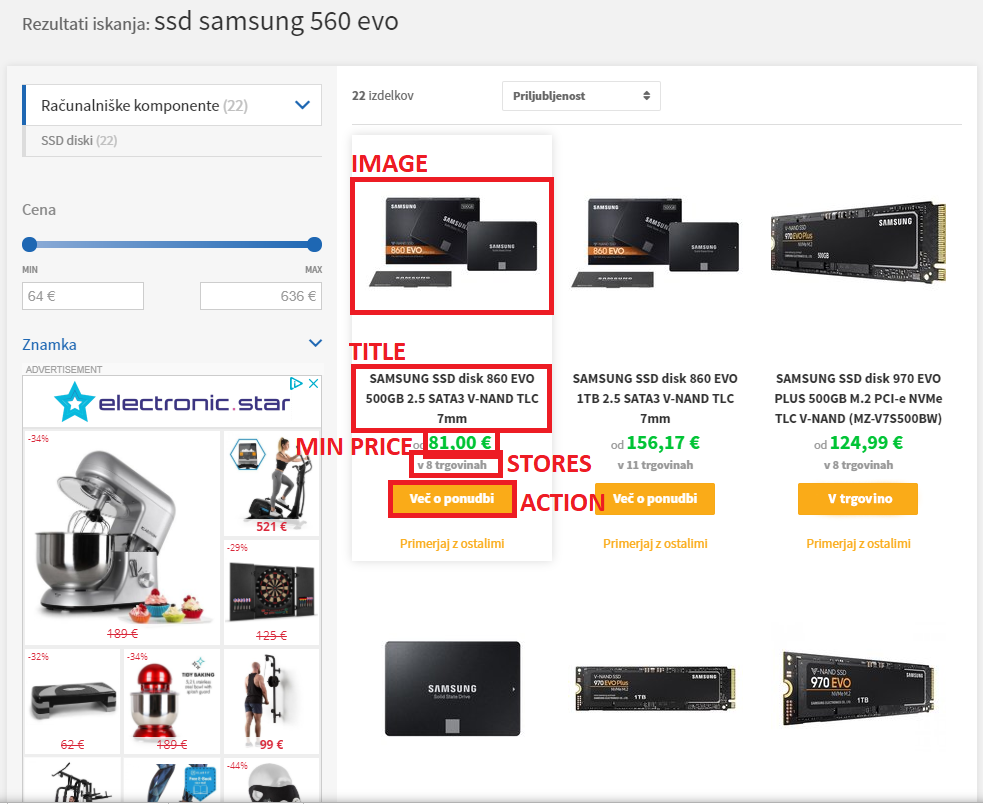
\includegraphics[width=1\columnwidth]{ceneje.png}
    \caption{Web site ceneje.si with tagged fields that we used for extraction of web content.}
    \label{fig_ceneje}
\end{figure}


\section{Regular Expressions Implementation}

Bellow is the list of all regular expressions that were used on the target web pages.

\subsection{rtvslo.si}
\begin{verbatim}
	Title: 			<h1>(.*?)</h1>
	SubTitle:		<div class=\"subtitle\">(.*?)</div>
	Lead:			<p class=\"lead\">(.*?)</p>
	Content:		<div class=\"article-body\">(.*?)</div>[ ]
*<div class=\"article-column\">
	Author: 		<div class=\"author-name\">(.*?)</div>
	PublishedTime:	<div class=\"publish-meta\">(.*?)<br>
\end{verbatim}

\subsection{overstock.com}
\begin{verbatim}
	Title(s):		<td valign=\"top\">\W*<a.*?PROD_ID=([0-9]+)\"
.*?<b>(.*?)</b></a>
	Content(s):		<td valign=\"top\">\W*<a.*?PROD_ID=([0-9]+)
\".*?<span class=\"normal\">(.*?)<br>	
	ListPrice(s):		<td valign=\"top\">\W*<a.*?PROD_ID=
([0-9]+)\".*?<s>(.*?)</s>
	Price(s):		<td valign=\"top\">\W*<a.*?PROD_ID=([0-9]+)
\".*?<span class=\"bigred\"><b>(.*?)</b>
	Saving(s):
	SavingPercent(s):	<td valign=\"top\">\W*<a.*?PROD_ID=
([0-9]+)\".*?<span class=\"littleorange\">(.*?) \((
[0-9]{0,2}\%)\)</span>		
\end{verbatim}

\subsection{mimovrste.si}
\begin{verbatim}
	Title:			<h3.*?>(.*?)</h3>
	Description:		<p.*?itemprop=\"description\".*?>(.*?)<a
	OldPrice:		<del.*?class=\"rrp-price\".*?>(.*?)</del>
	Price:			<b class=\"pro-price.*?>(.*?)</b>
	Availability:		<a data-sel=\"availability-detail\".*?>
(.*?)</a>
	Tags:			<em class=\"label.*?>(.*?)</em>
	Savings:		<div class=\"label--round-sale.*?>(.*?)</div>
\end{verbatim}

\subsection{ceneje.si}
\begin{verbatim}
	Image(s):		<div class=\"innerProductBox\">.*?<img.*?
alt=\"(.*?)\".*?src=\"(.*?)\"
	Titles(s):		<div class=\"innerProductBox\">.*?<img.*?
alt=\"(.*?)\".*?<h3>\W*<.*?>(.*?)</.*?>
	MinPrice(s):		<div class=\"innerProductBox\">.*?<img.*?
alt=\"(.*?)\".*?<b>(.*?)</b>
	Store(s):		<div class=\"innerProductBox\">.*?<img.*?
alt=\"(.*?)\".*?class=\"qtySellers\">\W*<b>(.*?)</b>
	Action(s):		<div class=\"innerProductBox\">.*?<img.*?
alt=\"(.*?)\".*?<div class=\"rBox\">\W*<.*?>(.*?)</.*?>
\end{verbatim}

\section{XPath Implementation}

Bellow are the lists of XPath expressions for every of the targeted pages.


\subsection{rtvslo.si}
\begin{verbatim}
	Title:			//*[@id=\"main-container\"]/div[3]/div/header/
h1/text()
	SubTitle:		//*[@id=\"main-container\"]/div[3]/div/
header/div[2]/text()
	Lead:			//*[@id=\"main-container\"]/div[3]/div/header/
p/text()
	Content:		string(//*[@id=\"main-container\"]/div[3]/div/
div[2])
	Author:		//*[@id=\"main-container\"]/div[3]/div/div[1]/
div[1]/div/text()
	PublishedTime:	//*[@id=\"main-container\"]/div[3]/div/
div[1]/div[2]/text()[1]
\end{verbatim}

%TODO: FIND IF THIS CAN BE SIMPLIFIED!
\subsection{overstock.si}
\begin{verbatim}
	Title(s): 		/html/body/table[2]/tbody/tr[1]/td[5]/
table/tbody/tr[2]/td/table/tbody/tr/td/table/tbody/
tr[" + str(i) + "]/td[2]/a/b/text()
	Content(s):		/html/body/table[2]/tbody/tr[1]/td[5]/
table/tbody/tr[2]/td/table/tbody/tr/td/table/tbody/
tr[" + str(i) + "]/td[2]/table/tbody/tr/td[2]/span/text()
	ListPrice(s):		/html/body/table[2]/tbody/tr[1]/td[5]/
table/tbody/tr[2]/td/table/tbody/tr/td/table/tbody/
tr[" + str(i) + "]/td[2]/table/tbody/tr/td[1]/table/
tbody/tr[1]/td[2]/s/text()
	Price(s):		/html/body/table[2]/tbody/tr[1]/td[5]/
table/tbody/tr[2]/td/table/tbody/tr/td/table/tbody/
tr[" + str(i) + "]/td[2]/table/tbody/tr/td[1]/table/
tbody/tr[2]/td[2]/span/b/text()
	Saving(s):			
	SavingPercent(s):	/html/body/table[2]/tbody/tr[1]/td[5]/
table/tbody/tr[2]/td/table/tbody/tr/td/table/tbody/
tr[" + str(i) + "]/td[2]/table/tbody/tr/td[1]/table/
tbody/tr[3]/td[2]/span/text()
\end{verbatim}

%TODO: FIX TAGS BELLOW!
\subsection{mimovrste.si}
\begin{verbatim}
	Title:			//*[@id=\"content\"]/div/article/div[1]/
section[2]/h3/text()
	Description:		//*[@id=\"content\"]/div/article/div[1]/
section[2]/p[2]/text()
	OldPrice:		//*[@id=\"content\"]/div/article/div[1]/
section[2]/div[3]/div[1]/div[1]/div/del/text()
	Price:			//*[@class=\"price-wrapper\"]/div[1]/
div[1]/b/text()
	Availability:		//*[@class=\"delivery-wrapper\"]/a/
text()
	Tags:			//*[@id=\"content\"]/div/article/div[1]/
section[2]/p[1]/em[" + str(i) + "]/text()
	Savings:		//*[@id=\"content\"]/div/article/div[1]/
section[2]/div[3]/div[1]/div[2]/text()
\end{verbatim}

\subsection{ceneje.si}
\begin{verbatim}
	Image(s):		//*[@id=\"productGrid\"]/div[" + str(i) + "]
/div/div[1]/a/img/@src
	Title(s):		//*[@id=\"productGrid\"]/div[" + str(i) + "]
/div/div[2]/h3/a/text()
	MinPrice(s):		//*[@id=\"productGrid\"]/div[" + str(i) + "]
/div/div[2]/p/a[1]/b/text()
	Store(s):		//*[@id=\"productGrid\"]/div[" + str(i) + "]
/div/div[2]/p/a[2]/b/text()
	Action(s):		//*[@id=\"productGrid\"]/div[" + str(i) + "]
/div/div[3]/a/text()
\end{verbatim}


\section{Automatic Web Extraction Implementation}

\subsection{Pseudo code}

In our approach we first generated DOM structures from both input HTML pages.
Then we cleaned them by removing any <head>, <style> and <script> tags.
After that the auto\_ex function was called to produce a union--free regular expression.
When checking for node mismatches we mainly relied on the type of tag the node represented, the id of the node, if it didn't contain more than 3 numbers which generally described an ad node, and sequential attributes of the tag to determine if the two nodes in separate trees are the same.
The pseudo code of the function is described bellow. 

\begin{verbatim}
	def auto_ex(tree1, tree2):
		for child in tree1:

	        # Check if there is any node on count position
 in tree2
	        if count >= len(node_2.getchildren()):
	            wrapper += "(<" + str(child.tag).upper() 
+ "... >)?"
	            continue

	        target = node_2.getchildren()[count]

	        # Handle tag mismatches
	        if mismatch(child, target):
	            if contains(node_2, count, child):
	                wrapper += "(<" + target.tag.upper() 
+ "... >)?"
	                count += 1
	                target = node_2.getchildren()[count]
	            else:
	                wrapper += "(<" + str(child.tag).upper()
 + "... >)?"
	                continue
	        # Add starting tag
	        new_tag = "<" + str(child.tag).upper() + ">"

	        # Add text inside of the tag
	        if child.text is not None:
	            new_tag += get_smt(child.text, target.text)

	        # Handle children of this node
	        new_tag += auto_ex(child, target)

	        # Add a closing tag
	        new_tag += "</" + str(child.tag).upper() + ">"

	        # Handle text after the current node
	        if child.tail is not None:
	            tail = child.tail
	            if len(tail) > 0:
	                new_tag += get_smt(tail, target.tail)

	        # Replace multiple occurrences with a special
tag
	        if new_tag == prev_tag:
	            wrapper = re.sub(new_tag + "$", "(" + 
new_tag + ")+", wrapper)
	            continue

	        wrapper += new_tag

	        prev_tag = new_tag
	        count += 1

	        # If this is the last node in tree1 but there are
 still nodes in tree2 this one must be optional
	        if node_exists(tree2, level, count):
	            wrapper += "(<" + node_that_exists_in_tree2
 + "... >)?"

    return wrapper
\end{verbatim}

\subsection{Results}

\subsection{rtvslo.si}
\begin{verbatim}
	%TODO: Results
\end{verbatim}

\subsection{overstock.com}
\begin{verbatim}
	%TODO: Results
\end{verbatim}

\subsection{mimovrste.si}
\begin{verbatim}
	%TODO: Results
\end{verbatim}

\subsection{ceneje.si}
\begin{verbatim}
	%TODO: Results
\end{verbatim}

\section{Conclusion}

We were successful in implementing all of the above listed approaches and have gathered good results.
Our automatic web extraction approach could of course be improved with additional information gathered from other articles that tackle with the same problems or with testing the algorithm on more websites.

\bibliographystyle{IEEEtran}
\bibliography{main}

\end{document}
